\chapter{Experimentos}\label{sec:experiments}
%======================================================================================
No presente trabalho, nos concentramos no objetivo proposto descrito na Seção~\ref{sec:objetivo}.

\section {Procedimento}
Primeiramente, filmamos algumas esculturas utilizando a câmera de um {\it smartphone} convencional na resolução de 1920x1080 pixels. Esta filmagem foi realizada varrendo toda (ou a maioria) da superfície da escultura em 360 $^{circ}$ com o intuito de ter toda a escultura reconstruída \ref{fig:procedimentoscan}.
Após isso, fizemos mais alguns vídeos, pegando alguns pontos que possuíam mais detalhes e que, com uma única varredura, não era capaz de reproduzir uma boa reconstrução.

\begin{figure}[!h]
	\centering
	%   \includegraphics[width=1.0\linewidth]{figs/3d-curve-sketch/system-diagram.eps}
	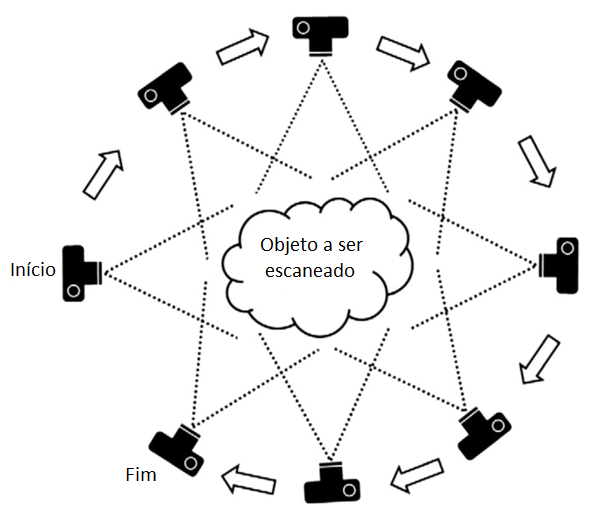
\includegraphics[width=0.5\linewidth]{figs/procedimentoscan.png}
	\caption{%
	Exemplo de como foi realizada a varredura da escultura
	%\cite{Cui:Theobalt:etal:PAMI2013,Pajdla:etal:ICCV2011}.
	}\label{fig:procedimentoscan}
\end{figure}
Com este material, foram feitos "cortes" em determinados {\it frames} do vídeo, com atenção para não pegar {\it frames} muito juntos, pois aumenaria o número de correspondências ambíguas entre as imagens e com isso, o processamento da reconstrução demoraria mais. E não pegar {\it frames} muito distantes, o que ocorreria o inverso, com menos correspondências, ficariam buracos na reconstrução. Como descrito na Seção \ref{sec:mve}.
Com isso em mente, foram reconstruídas duas esculturas: uma com um único vídeo, usando o VisualSfM, totalizando 200 imagens e outra com dois vídeos, com o MVE, com dois vídeos, que, ao cortá-los, totalizou cerca de 280 imagens.

%
%Nosso sistema prático foi projetado para C++ usando as bibliotecas de visão 
%computacional VXL e VXD~\cite{vxl,vxd}. A linguagem C++ é rápida e escalável, e muitas
%vezes é a única solução para as grandes quantidades de processamento de vídeo que
%visamos. Além disto, escolhemos utilizar uma solução baseada em VXL por ser
%amplamenta utilizada na indústria, pela sua suite de testes e, também, por
%prover a opção de utilizar OpenCV caso necessário. A VXL é internamente utilizada
%por empresas como a General Electrics, a Vision Systems Inc, a Google, e uma
%série de startups e universidades, para sistemas de visão maiores e mais
%experimentais do que o OpenCV.
%
%Na prática, no entanto, foram apenas implementados os filtros treinados finais e
%os sinais (\emph{features}) em C++, com base no código Matlab de referência
%por~\etal~\cite{Guo:etal:CVPR14,Guo:etal:PAMI2017:submitted}. Nosso código 
%C++ é aberto na biblioteca VXD e já foi usado pela
%Brown University e outros pacotes~\cite{Yuliang:edge:detection:github}. Decidimos 
%manter o treinamento dos
%classificadores topológicos de fragmentos de curva em Matlab, pois queríamos
%experimentar muito com ele usando a interatividade fornecida por essa linguagem
%``lab''. O código Matlab é baseado no código original de
%Guo~\etal~\cite{Guo:etal:CVPR14,Guo:etal:PAMI2017:submitted}.
%
%O processamento C++ foi implementado em paralelo, usando um nível UNIX
%de granularidade de comunicação. Na implementação atual, cada processo atua em
%dados de um único quadro de vídeo separadamente, em um único nó, usando
%múltiplos núcleos. O paralelismo de nível de processo é programado de forma
%flexível e programável para pesquisa, o GNU
%Parallel~\cite{Tange:GNU:Parallel:USENIX2011}, que também pode usar
%múltiplos nós como no MPI.
%
%Este nível de granularidade foi mais do que suficiente para acelerar nosso
%processamento de vídeo e protótipo do sistema, mas \emph{multithreading} através do
%paradigma de fluxo de dados também é uma possibilidade, pois usamos a
%mesma tecnologia subjacente que o sistema 3D Curve Sketch
%Multithread~\cite{Fabbri:Kimia:CVPR10}.
%
%Além disso, o paralelismo de nível de processo simples é bastante poderoso,
%robusto, programável e extensível, ao longo da tradição UNIX de dividir um
%sistema grande em pequenos programas independentes. É favorável à distribuição
%futura através do MPI e tecnologias relacionadas, enquanto o código interno para
%cada processo é acessível por níveis de granularidades mais finos através do
%CUDA; Os processos podem acelerar a comunicação através da memória ou dos pipes
%compartilhados em vez da abordagem baseada em arquivos atual. O custo da criação
%do processo é insignificante cada vez que os dados são lidos por quadro, uma vez
%que as imagens e o vídeo multivisão são muito ``big data''.
%
%\section {Processamento inicial}
%
%Cada um dos quatro vídeos de 3min é convertido em 182 arquivos de imagem PNG, um
%por quadro, usando o software de processamento de vídeo multithreaded de baixo nível
%FFmpeg~\cite{FFmpegurl}. Isso é adequado para a prototipagem de uma solução de pesquisa, e
%também para uma solução final de processamento em lote (\emph{batch}). Um sistema de produção
%poderia explorar formas de decodificar o vídeo \emph{on-the-fly} usando hardware, se o
%objetivo é o processamento online em tempo real. No entanto, dada a imagem maior
%que nosso rastreador de borda será usado dentro de um sistema de reconstrução 3D
%que usa muitos quadros globalmente no vídeo, extrair quadros em arquivos de
%imagem não é o gargalo.
%
%%\begin{figure}
%%  \centering
%%  \includegraphics[width=\linewidth]{figs/representative-frames.pdf}
%%  \caption{
%%    Video frames representative of the sea state, extracted from the first camera.}
%%  \label{fig:frames}
%%  \ReduceAfterCaptionfigspace
%%\end{figure}
%
%\begin{figure}[ht]
%  \caption{Etapa de pré-processamento de vídeo: regiões de interessse (a, c) e
%    correção de gama automática opcional (d) otimizamos esse problema, mas não
%    é necessário no sistema atual. O sinal de onda está concentrado nos
%    primeiros 40/255 níveis de cinza (16\%) (b). Veja os materiais
%    suplementares para os vídeos.}
%  \centering
%  \includegraphics[width=\linewidth]{figs/roi-gamma.pdf}
%  \source{O autor, 2017.}
%  \label{fig:roigamma}
%  \ReduceAfterCaptionfigspace
%\end{figure}
%
%\section {Processamento de Imagem}
%
%Para permitir o estudo científico dos padrões nos vídeos, recortamos os quadros
%em regiões de interesse (ROIs). As coordenadas desses ROIs atualmente são
%escritas manualmente para processamento paralelo, de modo que as regiões se
%sobrepõem, tanto quanto possível, entre as câmeras.
%
%A informação desejada nos vídeos está concentrada nos primeiros 40 níveis de
%cinza de 255 (16\%), Figura~\ref{fig:roigamma}. Portanto, foram automaticamente 
%recortados e, opcionalmente, realizado
%ajuste automático de gama em cada quadro em paralelo, usando
%ImageMagick~\cite{ImageMagickurl} e
%GNU Parallel~\cite{Tange:GNU:Parallel:USENIX2011}, 
%Figura~\ref{fig:roigamma}. O ImageMagick é conhecido por priorizar a qualidade
%da imagem sobre a velocidade; Na prática, o uso de sua API a partir de C++ não
%resultaria em benefício de desempenho significativo, ao mesmo tempo em que
%diminuiria a robustez do sistema.
%
%Em nossas experiências, observamos que a extração da curva é robusta o
%suficiente para não requerer este passo de ajuste automático de gama. No entanto, incluímos aqui
%para relatar esta descoberta, e também que selecionamos cuidadosamente
%para este conjunto de dados e pode ser um passo útil para outros tipos de
%processamento. É também o melhor filtro automático para fins de visualização
%desses vídeos, entre muitos que avaliamos. O resultado de que a extração da
%curva foi comprovada robusta com um contraste tão fraco em nossos vídeos é um testemunho
%do poder da abordagem do processamento de imagens usando descontinuidades de
%sombreamento, em vez de regiões de luminosidade suave.
%
%\section{Detecção de borda}
%\begin{figure}
%  \caption{Detector de borda de terceira ordem aplicado a um quadro de vídeo.
%    Observe que a informação bruta é puramente localizada nas bordas, com muitos
%    ruídos detectados em artefatos de compressão. O quadro é ajustado em gama
%    (superior), mas nossas experiências mostraram que o detector de borda é
%    robusto o suficiente para funcionar diretamente sem ajuste de gama.}
%  \centering
%  \includegraphics[width=\linewidth]{figs/third-order-sample-zoom.pdf}
%  \source{O autor, 2017.}
%  \label{fig:3o:zoom}
%  \ReduceAfterCaptionfigspace
%\end{figure}
%
%O detector de borda descrito na Seção~\ref{sec:edge:detection} foi codificado em um programa
%independente para ser aplicado em paralelo em cada quadro usando o GNU Parallel.
%Os parâmetros são armazenados em um arquivo XML, e um shell script foi
%escrito para construir e executar o comando GNU Parallel apropriado para
%arquivos PNG de entrada. A saída é um mapa de borda de subpixel no formato EDG, um
%formato de arquivo de texto compactado com gzip com extensão '\texttt{.edg.gz}'.
%
%Conforme mencionado no Capítulo~\ref{sec:cfrag:extraction}, nossa estratégia é
%estabelecer um limiar de
%baixo contraste para que possamos ter dados de borda brutos com alta cobertura,
%mas muitos falsos positivos a serem filtrados por consistência geométrica pelos
%próximos módulos na pipeline de processamento. A Figura~\ref{fig:3o:zoom} mostra uma amostra
%da detecção de borda inicial com ponto de operação de cobertura ideal para
%nossa aplicação. Observamos que neste limite obtemos alto nível de detalhes nas
%ondas, mas também detectamos muitos artefatos de compressão de vídeo para serem
%removidos mais tarde.
%
%Percebe-se como a imagem de entrada possui bordas muito longas
%geometricamente consistentes com baixo contraste, o que é outra razão pela qual
%precisamos definir os limiares de contraste iniciais muito baixos para permitir
%que o algoritmo de agrupamento geométrico faça o trabalho de escolhê-los. Outro
%benefício de confiar na filtragem geométrica em um nível superior é que a
%estratégia funciona para a maioria dos tipos de imagens sem ter que ajustar
%limiares - basta deixá-los baixos. Isso é confirmado por nossos experimentos,
%onde observamos que o filtro de ajuste automático de gama não é necessário ao iniciar o sistema
%com limiares de contraste muito baixos. Após extensas experiências iniciais, foram
%consertados os parâmetros do detector de borda de terceira ordem de acordo com
%as seguintes regras:
%\begin{itemize}
%  \item Um limite de contraste de '20\% 'foi suficiente para a maioria das
%    aplicações
%  \item Um parâmetro de suavização $\sigma = 2px$ foi considerado o mais útil para
%    aplicações de reconstrução em 3D, mas $\sigma = 3px$ apresentou melhores resultados
%    visuais e uma imagem mais limpa. Esse parâmetro afeta a escala das bordas,
%    mas também introduz a imprecisão de localização, a qual a calibração é
%    sensível. A localização poderia potencialmente ser corrigida ao combinar as
%    bordas em $\sigma = 3px$ com as bordas calculadas por uma escala inferior
%    $\sigma = 2px$,
%    de uma forma multi escala, mas, da nossa experiência, os benefícios
%    potenciais parecem baixos.
%\end{itemize}
%A Figura~\ref{fig:3o:zoom} mostra um resultado de detecção de borda de amostra
%para $\sigma = 3px$.
%
%\section{Extração do contorno inferior}
%Realizamos experimentos extensivos para calcular a saída do agrupamento de borda
%simbólico e suas
%variantes~\cite{Tamrakar:Kimia:ICCV07,Guo:etal:CVPR14,Guo:etal:PAMI2017:submitted}, 
%conforme descrito no Capítulo~\ref{sec:cfrag:extraction}, de início sem o uso
%de qualquer aprendizagem de máquina. Um exemplo de
%quadro do melhor resultado que conseguimos é dado na Figura~\ref{fig:sel:best},
%Seção~\ref{sec:main:results} abaixo. Veja os quatro vídeos no material
%suplementar para perceber as curvas acompanhadas.
%Neste nível de extração de fragmentos de curva, nosso objetivo é produzir alta
%precisão, e secundariamente uma cobertura máxima sem sacrificar a precisão. Alta
%precisão é obrigatória para o estágio inicial das aplicações 3D, uma vez que os
%\emph{outliers} podem sobrecarregar o sistema de inicialização (calibração da câmera e
%correspondência multivisão estéreo); cobertura é desejável, mas apenas para
%completar as reconstruções em uma segunda etapa de reconstrução em 3D.
%
%Em nossas experiências, realizamos um estudo de parâmetros sobre os muitos
%parâmetros internos ao código de extração de fragmentos de curva. A conclusão
%foi que apenas o limiar de comprimento (extensão da consistência geométrica) foi
%significativo. Para uso na primeira fase da reconstrução em 3D, empregou-se um
%limiar de comprimento mais agressivo de 160px (ou seja, apenas foram mantidas
%curvas com comprimento maior ou igual a 160px), representadas na
%Figura~\ref{fig:sel:best}.
%Para tentar aumentar a cobertura, tentamos um limite de comprimento de 80px, mas
%houve mais \emph{outliers} que se ligam aos padrões de ruído de
%compressão de fundo. Para os estágios posteriores da reconstrução,
%gostaríamos de conseguir uma maior cobertura. É por isso que exploramos a abordagem
%baseada em aprendizagem supervisionada como descrito na próxima seção. Outra
%situação em que precisamos melhorar esses resultados é quando o padrão de água
%fica mais quebrado, caso em que o sistema precisa ser robusto o suficiente para
%lidar com curvas menores (assim, maior cobertura) com maior precisão.
%
%Os estágios posteriores das aplicações de reconstrução 3D são capazes de
%filtrar contornos falso-positivos, exigindo que sejam consistentes em várias
%imagens e vídeos. Portanto, em princípio, o sistema pode se beneficiar de maior
%cobertura e menor precisão. Isso, no entanto, supera o custo computacional do
%sistema de correspondência multivisão estéreo. Em cenas desafiadoras, como em
%imagens aquáticas, existem muitos padrões repetitivos, de forma que a alta precisão e
%a cobertura possam ser cruciais como entrada.
%
%\section{Extração de contorno baseada em aprendizagem}
%\begin{figure}[h]
%  \caption{Filtros de união e quebra de contorno geométrico: exemplos de efeitos.}
%  \centering
%  \includegraphics[width=\linewidth]{figs/break-merge-zoom.pdf}
%  \source{O autor, 2017.}
%  \label{fig:break:merge:sample}
%  \ReduceAfterCaptionfigspace
%\end{figure}
%
%Os filtros de quebra e união geométricos descritos no
%Capítulo~\ref{sec:cfrag:extraction} foram aplicados
%na tentativa de aumentar o nível de detalhes (cobertura) nos padrões de ondas,
%minimizando falsos positivos (alta precisão). A
%Figura~\ref{fig:break:merge:sample} ilustra os efeitos
%dos filtros de união e quebra em um quadro de imagem real do tanque de ondas de
%água. A Figura~\ref{fig:break:merge:sample} ilustra os efeitos de cada etapa aplicada em seqüência,
%incluindo a união, quebra e remoção baseada em classificação, usando o conjunto de
%treinamento descrito em~\ref{sec:generic:datasets}.
%\begin{figure}
%  \caption{Resultados da amostra de estágios de aprendizagem de máquinas
%  supervisionados.}
%  \centering
%  \includegraphics[width=\linewidth]{figs/learned-results-sample.pdf}\hspace{-1em}
%  \legend{(a) Entrada da geometria do agrupador de borda simbólica
%    crua com alta cobertura; (b) Filtro de quebra aprendido a partir de
%    imagens genéricas naturais (c) Filtro de ranqueamento/classificação aprendido com imagens
%    naturais; (d) Filtro de união aprendido com imagens naturais genéricas.}
%  \source{O autor, 2017.}
%  \label{fig:learned:samples}
%  \ReduceAfterCaptionfigspace
%\end{figure}
%
%
%%\todo{Describe the results using Dayany dataset}
%%\todo{Incluir dados acima na apresentação}
%
%\section{Resultados principais}\label{sec:main:results}
%
%Nossos melhores resultados sem aprendizado são mostrados
%num instante de tempo na Figura~\ref{fig:sel:best}. Estes já são suficientes para entrar em um
%pipeline de reconstucção
%3D~\cite{Fabbri:Kimia:CVPR10,Usumezbas:Fabbri:Kimia:ECCV16,Usumezbas:Fabbri:Kimia:CVPR17}. 
%Consulte os vídeos no material suplementar para analisar todos os
%quadros. Ao aplicar toda a pipeline de processamento aos quatro vídeos de
%entrada, conseguimos melhorar a cobertura sem perda relativa de precisão,
%Figura~\ref{fig:learned:final}.
%
%%/todo{incluir esse dados na apresentação}
%
%\begin{figure}
%  \caption{Os melhores resultados de curva agrupada não supervisionados para
%    reconstrução em 3D e fotogrametria. Os resultados exibem uma alta precisão,
%    mas a cobertura pode ser melhorada (dados faltantes). Veja os vídeos nos
%    materiais suplementares.}
%  \centering
%  \includegraphics[width=\linewidth]{figs/raw-sel-best-result.png}
%  \source{O autor, 2017.}
%  \label{fig:sel:best}
%  \ReduceAfterCaptionfigspace
%\end{figure}
%
%\begin{figure}
%  \caption{Resultados finais de alta cobertura em um quadro de um dos quatro
%    vídeos. Veja o material suplementar para os vídeos.}
%  \centering
%  \includegraphics[width=\linewidth]{figs/final-high-recall-results.pdf}
%  \source{O autor, 2017.}
%  \label{fig:learned:final}
%  \ReduceAfterCaptionfigspace
%\end{figure}
